\section{Experiments}
\label{experiments}

Our experimental evaluation of a prototype implementation of POLAR studies its general applicability and performance characteristics with a variety of benchmarks. After describing the prototype and experimental setting, we use various micro benchmarks to evaluate the behavior of different strategies and parameters and conduct end-to-end performance comparisons with DuckDB~\cite{RaasveldtM19}, Postgres~\cite{DBLP:conf/sigmod/StonebrakerR86}, SkinnerDB~\cite{TrummerWMMJA19, TrummerWWMMJAR21}, SkinnerMT~\cite{WeiT22}, and Lookahead Information Passing~\cite{ZhuPSP17} in DuckDB. Our major findings are that: 
\begin{enumerate}
\item Non-invasive AQP yields robust end-to-end performance,
\item Offers substantial speedups for certain queries, especially on skewed benchmarks, and
\item Is already effective with small exploration budgets of $\leq$1\,\%. 
\end{enumerate}

\subsection{Experimental Setup}

\textbf{Prototype:} We implemented POLAR in DuckDB, a state-of-the-art OLAP DBMS. The prototype\footnote{We share our prototype and artifacts at \url{https://github.com/damslab/reproducibility}.}, including the different routing and selection strategies, is ~2500 LoC and requires minimal changes to the existing DuckDB code. The input to POLAR is a query plan produced by the DuckDB optimizer, which uses equivalence sets to estimate cardinalities~\cite{thesis/Ebergen22} and DPhyp~\cite{MoerkotteN08} for join ordering.  

\textbf{Evaluation System:} We conducted all experiments on a Lenovo ThinkSystem SR635 server with a single AMD EPYC 7443P CPU at $2.85$\,GHz (24 physical/48 virtual cores), 256\,GB DDR4 RAM at 3.2\,GHz, $1\times 480\,\text{GB}$ SATA SSD, $8\times 2\,\text{TB}$ SATA HDDs (data) and Mellanox ConnectX-6 HDR/200\,Gb Infiniband. We compiled the source code with clang-12 on Ubuntu 20.04.1.

\textbf{Benchmarks:} We evaluate POLAR on the Join Order Benchmark (JOB)~\cite{JoinOrderBenchmark}, Star Schema Benchmark (SSB)~\cite{SSB-ONeil2009-qs}, and a modified SSB with correlation and skew (SSB-skew), both with a scale factor of 100.
%
We introduce SSB-skew as a benchmark with SSB's applicability (long join pipelines, cf. Section~\ref{sec:potential-analysis}) but real-world data characteristics such as cross-correlations, skew, and clustered data. In SSB-skew, most customers are from the US and most suppliers are from Asia. Moreover, the \texttt{part} table references are skewed, so many lineitems belong to a few part categories and brands. The \texttt{lineorder} table is clustered by order date, with a recession of few orders in 1997 and a year of growth in 1998. Finally, the number of lineitems from suppliers in the United States increases over time. SSB-skew uses SSB's original queries except query set 1 (only one join).
%
We do not use TPC-H \cite{tpch} and JCC-H \cite{JCC-H} because (1) their optimal join orders are well-known and often tuned for, and (2) the join orders generated by DuckDB are mostly right-deep trees, not amenable to POLAR. We also considered the LDBC Social Network BI Workload~\cite{LDBC}, but LDBC requires advanced SQL features which are not supported by all systems we compare, and the DuckDB optimizer often generates pipelines with alternating joins and projections, which our prototype does not yet support (cf. Section~\ref{sec:limits}).
%

%%%%%%%%%%%%%%%%%%%%%%%
\subsection{Applicability Study}
\label{sec:potential-analysis}

\begin{table}[!t]
	\centering 
	\caption{Intermediate Tuple Reduction and Coverage of Amenable Piplines -- Total number of intermediate tuples and fraction of total execution time spent in amenable pipelines.}
	\vspace{-0.3cm} \setlength\tabcolsep{5pt}
	\begin{tabular}{lrrrr}
		\toprule
		\textbf{Benchmark} & \textbf{DuckDB} & \textbf{Routing} & \textbf{Static} & \textbf{Coverage}\\
		\midrule
		JOB &     107.49 M &      16.92 M &      25.84 M & 37 \%\\
		SSB &      86.65 M &      55.06 M &      57.83 M & 68 \%\\
		SSB-skew &     929.87 M &      25.15 M &     688.90 M & 97 \%\\
		\bottomrule
	\end{tabular}
	\label{tab:1_2_potential_savings}
\end{table}


In a first series of experiments, we aim to analyze the potential of POLAR by estimating the possible reduction in the number of intermediates with optimal routing strategies. These results serve as a baseline---in terms of an upper bound---for later experiments evaluating the quality of POLAR routing strategies. Furthermore, we also examine the time spent in amenable pipelines. Combining these measures allows estimating the overall potential.

\textbf{Potential Reduction of Intermediates:} Table~\ref{tab:1_2_potential_savings} shows the potential performance improvements achievable with adaptive join order switching. We calculated the potential improvement by measuring the number of intermediate results for all amenable pipelines using DuckDB's default join order, the best static join order for each pipeline, and an estimated optimal routing strategy. We determined this optimal value using a multiplexer debugging mode, routing each input chunk to every legal join order and measuring the minimal number of intermediates.
%
Table~\ref{tab:1_2_potential_savings} shows that dynamic tuple routing reduces the number of intermediates for all benchmarks but the potential improvement over an ideal static join order is most significant with skewed datasets. For JOB, the best static join order produces 25.84\,M tuples compared to 107.49\,M tuples from DuckDB's default join order. Dynamic routing further improves this number to 16.92\,M tuples. This result shows that a better static join order could improve JOB to a large extent without dynamic join order switching at runtime. For SSB, neither join order switching nor better join orders considerably improve the number of intermediates. The best static join order produces 578.23\,M tuples, a moderate improvement over the 747.67\,M tuples in the default DuckDB plan, and dynamic routing yields only a slight additional improvement to 547.40\,M tuples. DuckDB's near-optimal plan for SSB is expected because the benchmark contains well-behaved FK/PK joins and uniform, non-skewed data.
%
For SSB-skew, which includes correlation and skew, the potential for improvement is much higher. The default DuckDB join order produces 2690.05\,M tuples, while the best static join order produces 474.28\,M tuples. Tuple routing further decreases the optimal number of intermediates to 342.67\,M. Thus, SSB-skew benefits from routing about the same as JOB.

\begin{figure}[!t]
    \centering
    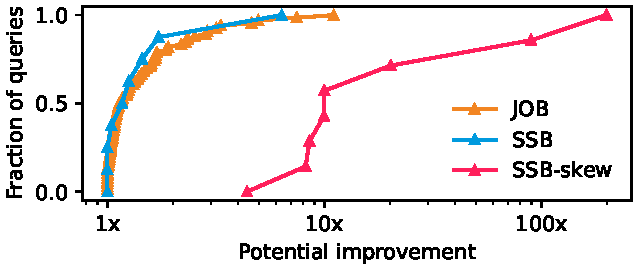
\includegraphics[width=0.95\linewidth]{figures/1_3_potential_query_improvements.pdf}
    \vspace{-0.4cm}
		\caption{Potential Query Performance Improvement.}
    \label{fig:1_3_potential_query_improvements}
		\vspace{-0.5cm}
\end{figure}

\textbf{Coverage of Amenable Pipelines:} Given DuckDB's default query plans, we measure each benchmark's total execution time and the time spent processing POLAR-amenable pipelines (\ie pipelines containing left-deep trees of two or more joins). Comparing the difference of these values yields the \textit{Coverage}, that is, the fraction of time spent in improvable pipelines. Note that the coverage also includes other operators from these pipelines, such as scans and aggregations, which POLAR cannot improve. The Coverage column in Table \ref{tab:1_2_potential_savings} shows that for JOB, DuckDB only spends 36\,\% of the processing time in POLAR-applicable pipelines. Consequently, almost two-thirds of the total execution time cannot be improved by POLAR. For SSB, DuckDB spends 73\,\% of the time in applicable pipelines, but many of them are dominated by large table scans and the joins only account for a small portion of the time. For SSB-skew, DuckDB spends almost all of the execution time (99\,\%) in applicable pipelines, and joins account for a large fraction of that time, providing substantial room for performance improvements.

\textbf{Potential Query Performance Improvement:} Furthermore, we aim to assess how much the runtime of individual queries could be improved. We estimate these improvements per query by multiplying the optimal number of intermediates with the coverage of amenable pipelines (assuming a linear relationship between tuple count reduction and execution time). Figure \ref{fig:1_3_potential_query_improvements} shows a cumulative distribution function over the potential performance improvements for all queries. Less than 10\,\% of the queries in JOB and SSB can be improved by more than 2x. Queries in SSB-skew show a much larger potential for improvement: over 40\,\% of the queries can be improved by more than an order of magnitude.

%%%%%%%%%%%%%%%%%%%%%%%
\subsection{Micro Benchmarks}
\label{sec:microbench}

\begin{figure}
    \begin{minipage}[t]{0.48\linewidth}
        \includegraphics[width=\linewidth]{figures/2_0_sample_size.pdf}
        \vspace{-0.65cm}
        \caption{\textsc{SelSampling} -- Relative Number of Intermediate of Best Join Order with Increasing Number of Samples.}
        \label{fig:2_0_sample_size}
    \end{minipage}%
        \hfill%
    \begin{minipage}[t]{0.48\linewidth}
        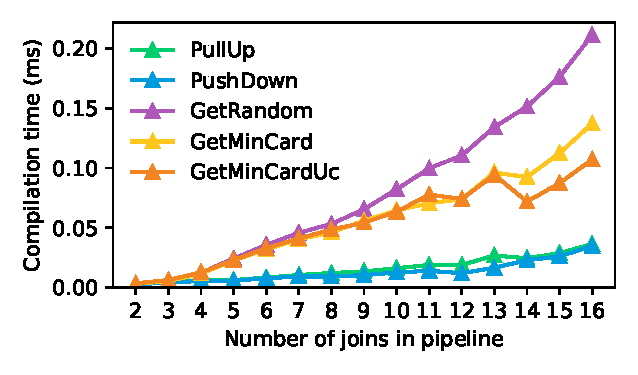
\includegraphics[width=\linewidth]{figures/2_2_enumeration_timings.pdf}
        \vspace{-0.65cm}
        \caption{Average Pipeline Compilation Time [ms] for Different Join Order Selection Strategies on SSB.}
				\label{fig:2_2_enumeration_timings}
    \end{minipage}
		\vspace{-0.5cm}
\end{figure}

\begin{figure*}[!t]
    \centering
    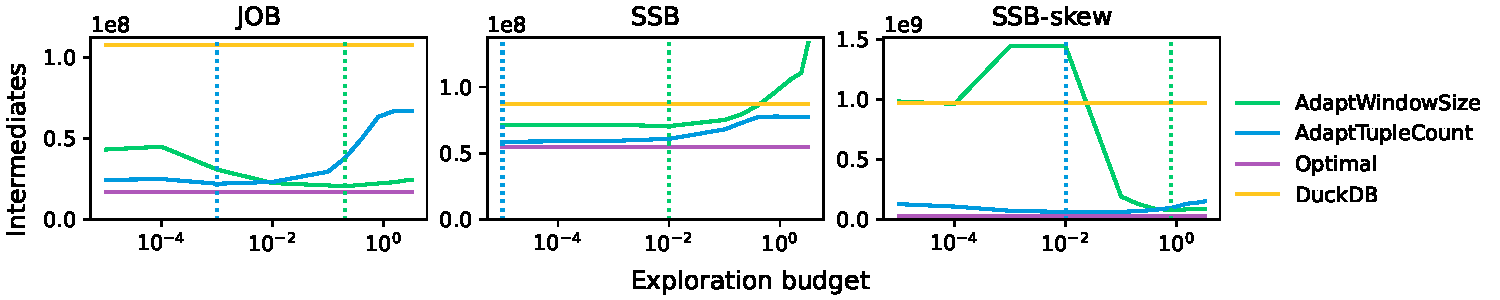
\includegraphics[width=0.95\textwidth]{figures/2_3_routing_adaptive.pdf}
		\vspace{-0.25cm}
    \caption{Exploration Budgets -- Number of Intermediate Tuples for Different Routing Strategies and Exploration Budgets (the dotted lines denote sweet spots in which the strategy generates minimal intermediates).}
    \label{fig:2_3_routing_adaptive}
		\vspace{-0.2cm}
\end{figure*}

In order to understand the trade-offs of different join selection and routing strategies, in a second series of experiments, we conduct several micro benchmarks regarding plan quality, compilation time, adaptivity, and runtime overhead. We also investigate the impact of the exploration budget on adaptivity and overhead. All micro benchmarks were executed single-threaded to isolate the effects.

\textbf{Sampling for Join Order Selection:} The \textsc{SelSampling} join selection strategy---introduced in Section~\ref{sec:paths}---systematically samples the space of cardinalities to find alternative join orders. We set the maximum join order count ${MAX}$ to $\card{J}!$ (\ie the number of possible orders for joins $J$, assuming clique queries). For an increasing number of samples, we determine the best possible outcome for the resulting join order set in terms of the intermediate optimum introduced in Section~\ref{sec:potential-analysis}. As a baseline, we exhaustively enumerate all possible join orders for each of the join pipelines. The results in Figure~\ref{fig:2_0_sample_size} show that even few samples allow for effective intermediate result reduction close to the level of exhaustive enumeration. By default, we set the sample count to 8 for the following experiments, which allows POLAR to find well-performing sequences of join paths while excluding unnecessary routing options. We used SSB-skew to test performance penalties induced by exhaustive enumeration and found deteriorations---despite no very long join pipelines---of up to 9\,\% with \textsc{AdaptTupleCount} and 1.5\,\% with \textsc{AdaptWindowSize} compared to \textsc{SelSampling} using 8 samples.

\textbf{Pipeline Compilation Time:} The time required to compile a POLAR pipeline is dominated by the join order selection. We measure this compilation time for the different join order selection strategies using pipelines with varying numbers of joins from SSB and SSB-skew as they contain the longest join pipelines. Figure~\ref{fig:2_2_enumeration_timings} compares the average pipeline compilation time with an increasing number of samples for \textsc{SelSampling} to the other strategies (again, with a join path limit of 8). Our results show that \textsc{SelSampling} generally takes longer to compile than the baselines, and its compilation time increases linearly until it reaches 8 join orders. After that, the increase becomes smaller as the strategy stops taking new samples if we already found $MAX$ distinct join orders. In any case, the compilation time for any pipeline is way below one millisecond and thus, negligible compared to the overall query processing times.

\begin{table}[!t]
  \centering
  \caption{Join Order Selection -- Total number of intermediates for POLAR pipelines with different selection strategies.}
  \vspace{-0.3cm}  \setlength\tabcolsep{3.5pt}
  \begin{tabular}{lrrrr}
    \toprule
    \textbf{Enumeration} & \textbf{JOB} & \textbf{SSB} & \textbf{SSB-skew} & \textbf{JOB-ldt}\\
    \midrule
    DuckDB* &     107.49 M &      87.36 M &     967.78 M &     248.30 M\\
    Optimal &      16.92 M &      55.06 M &      25.15 M & N/A\\
    \midrule
    \textsc{GetRandom} &      16.92 M &      55.06 M &      25.15 M &     156.64 M\\
    \textsc{GetMinCard} &      16.92 M &      55.06 M &      25.15 M &     189.47 M\\
    \textsc{GetMinCardUc} &      16.92 M &      55.06 M &      25.15 M &     189.44 M\\
    \textsc{PushDown} &      17.04 M &      59.78 M &      41.46 M &     208.83 M\\
    \textsc{PullUp} &      17.22 M &      59.88 M &      53.08 M &     210.73 M\\
    \bottomrule
  \end{tabular}
  \label{tab:1_1_sel_intms}
\end{table}


\textbf{Join Order Selection:} We further compare the quality of the join order selection strategies by comparing the actual number of intermediates to the optimal number, as described in Section~\ref{sec:potential-analysis}. To stress-test the different join order selection strategies, we also compared \textit{JOB-ldt}, which compiles the JOB queries using a greedy algorithm that only generates left-deep trees. Table~\ref{tab:1_1_sel_intms} summarizes the results.
For \textsc{GetMinCard} and \textsc{GetRandom}, we limit the number of join orders to 8, analogous to the \textsc{SelSampling}. For our set of benchmarks, even simple strategies such as \textsc{PushDown} yield competitive results that are close to the optimal number of intermediates. However, especially on SSB-skew, \textsc{PullUp} performs poorly. On JOB-ldt, \textsc{SelSampling} outperforms our baselines noticeably. Furthermore, as \textsc{GetMinCard} and \textsc{GetRandom} always produce the maximal number of join orders within the user-set limit and \textsc{PushDown} may include plans that are highly unlikely well-performing (such as an PK-FK join on a table without predicate as first join), \textsc{SelSampling} is the only strategy that may select small sets of useful, complementary join orders excluding unreasonable join paths. Therefore, we use \textsc{SelSampling} as POLAR's default.

\textbf{Join Order Initialization:} All routing strategies (excluding \textsc{Backpressure}) use a static number of tuples to initialize each of the join paths. In \textsc{AdaptWindowSize}, this number is also used to explore weaker paths after the initialization phase. To find a meaningful tuple count for path (re-)initialization, we conduct an experiment using the \textsc{InitOnce} strategy with an increasing number of initialization tuples and count the resulting number of intermediates. Figure~\ref{fig:2_5_init_tuple}  shows the results of that experiment. For JOB, 8 initialization tuples are already sufficient to determine join orders that produce less than 40\,\% intermediates incurred by DuckDB. However, for SSB, the number of intermediates gradually improves with the number of tuples. Therefore, we conservatively set the default initialization tuple count to 1024, which is also the chunk size in our DuckDB-based prototype.

\begin{figure}[!t]
    \centering
    \includegraphics[width=0.9\linewidth]{figures/2_5_init_tuple.pdf}
		\vspace{-0.5cm}
    \caption{Path Initialization -- Relative Number of Intermediates for Initial Input Tuple Counts using InitOnce.}
    \label{fig:2_5_init_tuple}
		\vspace{-0.5cm}
\end{figure} 

\textbf{Exploration Budgets:} For adaptive routing strategies, such as \textsc{AdaptTupleCount} and \textsc{AdaptWindowSize}, the quality of routing depends on the exploration budget. A higher budget allows the strategies to adapt better to path changes but also incurs larger overheads. To understand how the exploration budget affects the different workload characteristics, we execute JOB, SSB, and SSB-skew with exploration budgets from 0.001\,\% to 320\,\%. Figure \ref{fig:2_3_routing_adaptive} shows how the number of intermediates produced by the two adaptive routing strategies varies with increasing exploration budget. Both \textsc{AdaptTupleCount} and \textsc{AdaptWindowSize} achieve close to the optimal numbers of intermediates. However, the ideal exploration budgets differ for each benchmark. We attribute this effect to the differences in exploration potential, already observed in \ref{sec:potential-analysis}. 
%
While a larger budget only creates exploration overhead for SSB, exploration is crucial to find better join order alternatives for JOB and SSB-skew as the data characteristics change during query execution. \textsc{AdaptWindowSize} is especially sensitive to the exploration budget while \textsc{AdaptTupleCount} shows more robust behavior: small exploration budgets of up to 1\,\% are sufficient to obtain robust performance characteristics. Moreover, the sweet spots for \textsc{AdaptWindowSize} are generally higher than for \textsc{AdaptTupleCount} as the latter consistently keeps exploring alternative join orders even under small exploration budgets. As a result of this analysis, we set the exploration budget for \textsc{AdaptWindowSize} to 1\,\% and \textsc{AdaptTupleCount} to 0.1\,\% for the following experiments.

\begin{table}[!t]
	\centering
	\caption{Intermediate Results -- Total number of intermediates per routing strategy using tuned exploration budgets.}
	\vspace{-0.3cm} \setlength\tabcolsep{7.9pt}
  \begin{tabular}{lrrr}
	\toprule
		\textbf{Routing Strategy} & \textbf{JOB} & \textbf{SSB} & \textbf{SSB-skew}\\
		\midrule
		DuckDB &     107.49 M &      86.65 M &     929.87 M\\
		Optimal &      17.01 M &      55.06 M &      25.15 M\\
        \midrule
		\textsc{InitOnce} &      43.27 M &      67.84 M &     985.83 M\\
		\textsc{Opportunistic} &      24.48 M &      58.71 M &     655.38 M\\
		\textsc{AdaptTupleCount} &      22.05 M &      \textbf{58.70 M} &      \textbf{62.93 M}\\
		\textsc{AdaptWindowSize} &      \textbf{20.51 M} &      70.53 M &     77.92 M\\
		\textsc{Backpressure} &      41.94 M &     227.33 M &     651.14 M\\
		\bottomrule
	\end{tabular}
	\label{tab:2_4_routing_all}
\end{table}


\textbf{Routing Strategies -- Intermediates:} We compare the different routing strategies from Section~\ref{sec:routing_strategies} with regard to the number of intermediates they produce. Table~\ref{tab:2_4_routing_all} shows the results. \textsc{AdaptTupleCount} produces the least intermediates for JOB and shows competitive performance for SSB, whereas \textsc{AdaptWindowSize} produces the fewest intermediate results for SSB-Skew. \textsc{InitOnce} performs substantially worse than the adaptive strategies because it picks sub-optimal join orders whenever the initialization phase is not representative for the remaining data batches. This observation is especially pronounced for SSB-skew, where there are different optimal plans for different clusters of the data. The \textsc{Opportunistic} strategy performs best on SSB as it allows path switching without the overhead of exploration. \textsc{Backpressure} produces the most intermediate results because many executor threads process tuples through sub-optimal join orders.

\begin{table}[!t]
	\centering
	 \caption{Execution Time -- Total pipeline execution time per routing strategy [seconds].}
	 \vspace{-0.3cm}  \setlength\tabcolsep{11.4pt}
   \begin{tabular}{lrrr}
	  \toprule
		\textbf{Routing strategy} & \textbf{JOB} & \textbf{SSB} & \textbf{SSB-skew}\\
		\midrule
		DuckDB &      49.42 &       5.56 &      11.94\\
		\midrule
		\textsc{InitOnce} &      32.38 &       5.12 &      10.44\\
		\textsc{Opportunistic} &      31.44 &       6.78 &       9.40\\
		\textsc{AdaptTupleCount} &      31.44 &       7.46 &       6.50\\
		\textsc{AdaptWindowSize} &      31.02 &       5.21 &       5.36\\
		\textsc{Backpressure} &      68.35 &      14.26 &      20.65\\
		\bottomrule
	\end{tabular}
	\label{tab:3_1_pipeline}
\end{table}


\textbf{Routing Strategies -- Execution Time:} The performance of routing strategies does not solely depend on reducing intermediates. Another influential factor is how much adaptivity negatively affects vectorized execution. A high path switching rate can reduce intermediate buffer sizes, as explained in Section~\ref{sec:routing_strategies}. Therefore, we also examine the actual pipeline execution times for each routing strategy, as they are closely correlated with overall query execution time. Table \ref{tab:3_1_pipeline} shows the total pipeline execution time for different strategies using the tuned exploration budgets reported before. Since \textsc{AdaptWindowSize} trades path exploration granularity for better vectorization, the strategy performs best for exploration budgets that are below its sweet spots for minimal intermediates. Interestingly, the lowest number of intermediates does not necessarily lead to the lowest pipeline execution time. 
Despite producing more intermediates than its competitors on JOB and SSB, \textsc{AdaptWindowSize} outperforms each of them in all of our benchmarks. Therefore, we conclude that the strategy offers the best trade-off between reducing the number of intermediates and preserving good vectorized execution. Thus, we use \textsc{AdaptWindowSize} as POLAR's default routing strategy for the remainder of the experiments.

\begin{figure*}[!t]
    \centering
    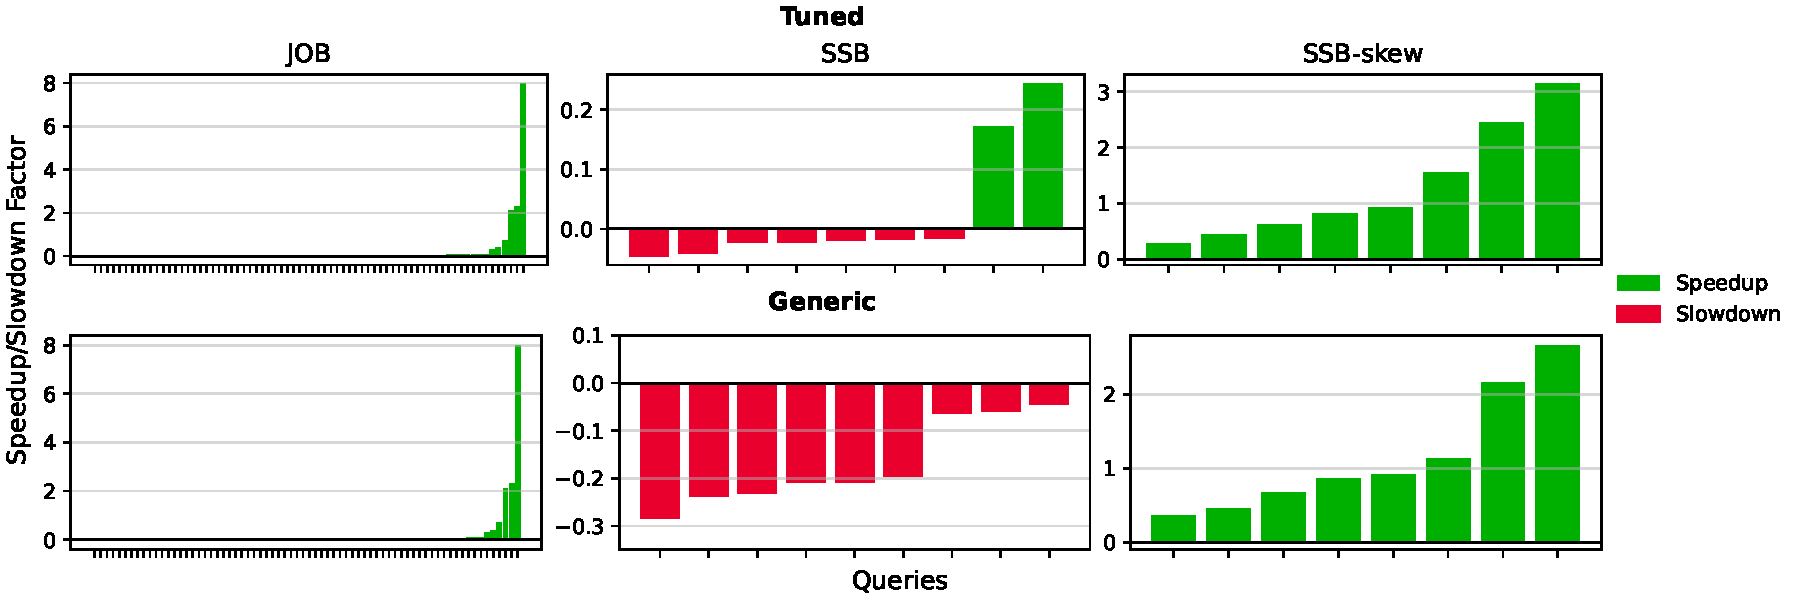
\includegraphics[width=0.99\textwidth]{figures/3_2_rel_gains.pdf}
    \vspace{-0.25cm}
    \caption{Individual Query Performance Impact -- Query performance changes between unmodified DuckDB and POLAR. A value of +1 indicates the query was 100\,\% faster (2x), and a value of -1 indicates a 100\,\% overhead (doubled execution time).}
    \label{fig:3_2_rel_gains}
		\vspace{-0.1cm}
\end{figure*}

\subsection{End-to-End Performance Comparison}
\label{sec:end-to-end}

Informed by the results from our micro benchmarks, we evaluate POLAR's end-to-end benchmark performance with \textsc{SelSampling} join order selection with 8 samples, an initialization tuple count of 1024, and the \textsc{AdaptWindowSize} routing strategy with a 1\,\% exploration budget for all benchmarks. In this context, we compare POLAR with DuckDB~\cite{RaasveldtM19}, a Lookahead Information Passing~\cite{ZhuPSP17} prototype on DuckDB, Postgres~\cite{DBLP:conf/sigmod/StonebrakerR86}, SkinnerDB (\ie Skinner-C)~\cite{TrummerWMMJA19}, and SkinnerMT~\cite{WeiT22}, a state-of-the-art AQP system, in both single- and multi-threaded configurations.

\begin{table}
	\centering
	\caption{Overall Performance Impact -- Single-threaded total execution time, and max execution time per query [seconds].}
		\vspace{-0.3cm} \setlength\tabcolsep{3.7pt}
   \begin{tabular}{lcccccc}
	  \toprule
		& \multicolumn{3}{c}{\textbf{Total Execution Time}} & \multicolumn{3}{c}{\textbf{Max. Query Time}}\\
         & JOB & SSB & SSB-skew & JOB & SSB & SSB-skew\\
		\midrule
		DuckDB & 135.5 & 7.8 & 12.2 & 10.7 & 1.1 & 3.6\\
        POLAR-G & 117.7 & 8.9 & 5.6 & 3.9 & 1.4 & 1.7\\
        POLAR-T & \textbf{117.7} & \textbf{7.5} & \textbf{5.6} & \textbf{3.9} & \textbf{0.9} & \textbf{1.7} \\
        Speedup & 1.15x & 1.04x & \textbf{\color{red}2.18x} & \textbf{\color{red}2.74x} & 1.22x & \textbf{\color{red}2.12x}\\
		\bottomrule
	\end{tabular}
	\label{tab:3_4_endtoend}
\end{table}


\begin{figure*}
    \centering
    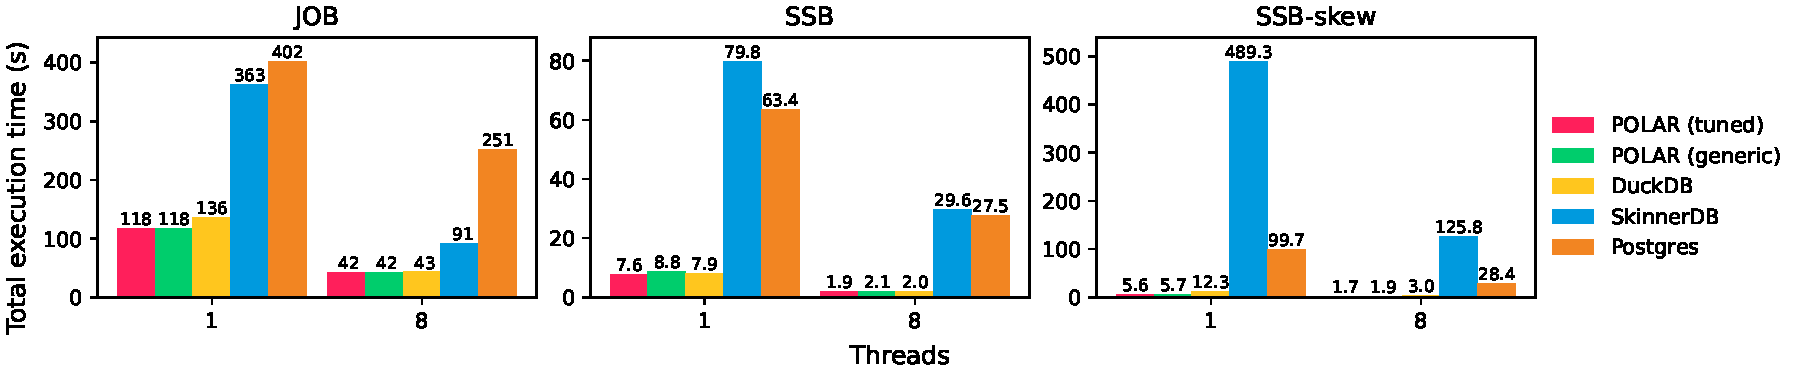
\includegraphics[width=0.99\textwidth]{figures/4_1_total.pdf}
    \vspace{-0.25cm}
    \caption{AQP System Comparison -- Total execution times for JOB, SSB, and SSB-skew, using 1 and 8 threads [seconds].}
    \label{fig:4_1_total}
		\vspace{-0.1cm}
\end{figure*}

\textbf{Overall Performance Impact:} Table~\ref{tab:3_4_endtoend} shows the total, end-to-end, single-threaded execution time and the maximum query execution times for DuckDB and POLAR on the different benchmarks. POLAR shows a slight overhead on SSB in total and maximum execution times and a moderate total execution time improvement of 1.16x on JOB. Moreover, POLAR shows a substantial 1.94x end-to-end improvement for SSB-skew and reduces the maximal query runtimes for JOB and SSB-skew by 2.78x and 2.98x, respectively. These results show that POLAR yields robust performance with substantial improvements for workloads on skewed data and only minor overhead for workloads where adaptation is not needed.

\textbf{Query Performance Impact:} Figure~\ref{fig:3_2_rel_gains} shows the speedups and slowdowns for each individual query with POLAR-amenable pipelines in JOB, SSB, and SSB-skew. A value of 1 indicates an improvement of 100\,\% (\ie half the execution time or 2x), whereas a value of -1 indicates double the execution time. For most JOB queries, POLAR has no positive or negative effect on the execution time. However, for a few queries, POLAR substantially reduces the execution time by up to 9x. The two queries with the largest speedups are also the longest-running queries in the benchmark. On SSB, the POLAR overhead increases the execution time for most queries, as expected, given how close to optimal the original plans are. However, one of the SSB queries also benefits from POLAR. Finally, almost all queries in SSB-skew improve with POLAR, up to 4x in one case. Therefore, POLAR achieves substantial performance and robustness improvements on non-uniform data and incurs only slight overhead for some queries on uniform data due to plan exploration and impact on vectorization at runtime. However, this moderate overhead is an acceptable price to pay for increased robustness, and the overhead could be further decreased when specializing POLAR to the underlying runtime system.

\textbf{Number of Intermediates:} The execution times of our baseline systems are strongly correlated with their underlying execution engines. Hence, we first conduct an experiment comparing the number of intermediates produced by their join orders. Table~\ref{tab:3_5_intermediates} shows the results. Note that SkinnerDB ran out-of-memory for SSB and SSB-skew. However, for JOB, SkinnerDB achieves a much lower number of intermediates than DuckDB, POLAR, and Postgres because it is not restricted to amenable pipelines. The comparison further shows that Postgres generally produces plans with fewer intermediates than DuckDB. Using POLAR reduces DuckDB's intermediates and outperforms Postgres by 1.4x on SSB-skew.

\input{tables/3_5_intermediates}

\textbf{AQP System Comparison:} To contextualize POLAR's performance, we compare POLAR, DuckDB, Postgres, SkinnerDB, and SkinnerMT, measuring the total execution time in single- and multi-threaded (8 threads) configurations. Additionally, we implemented a prototype of Lookahead Information Passing~\cite{ZhuPSP17} (LIP) in DuckDB to compare POLAR against a bitmap filtering approach. We allow SkinnerDB/MT to cache indexes on all join columns in memory to reduce its pre-processing time. We use Postgres 12.15 with indexes on all foreign key columns to prevent it from compiling aggressive plans with fatal nested-loop joins on unindexed join columns.
%
Figure~\ref{fig:4_1_total} shows that POLAR performs equally or better than DuckDB, SkinnerDB, and Postgres on almost all benchmarks. On SSB, POLAR shows a similar performance as DuckDB both single- and multi-threaded. On SSB-skew, POLAR outperforms DuckDB by 1.9x single-threaded and by 1.8x multi-threaded.
%LIP
While LIP shows equal execution times as POLAR on JOB, it performs slightly worse on SSB and substantially worse on SSB-skew. Regarding individual JOB queries, LIP shows occasional performance regressions of more than 2x, which is in line with experimental results from other bitmap filtering approaches \cite{DingCN20, LeeDNC23}. We account this performance gap to the large number of additional hash probes, lack of vectorization, and unstable bloom filter orderings.
%SkinnerDB/MT
SkinnerMT shows the best performance on JOB with multiple threads. However, SkinnerDB/MT run out-of-memory on SSB and SSB-skew. Previous experiments on SSB with scale factor 10 showed POLAR speedups of up to 15.6x over SkinnerDB (8 threads, 1.9\,s vs 29.6\,s) and around 3.9x over SkinnerMT. We attribute this to SkinnerDB/MTs custom join operator with tuple-at-a-time processing and the systems' ability to change the source table, which requires building hash tables for each relation.
%Postgres
As expected, Postgres shows much higher total execution times than POLAR and DuckDB, given its different target workloads and runtime system. These experiments demonstrate the benefits of a non-invasive, bounded-overhead system design in an engine designed for analytic workloads. In contrast to invasive AQP systems, POLAR favors reusing existing database components and original plans resulting in competitive performance and much greater performance robustness with modest overhead.
